\chapter{Results \& Discussion}
\label{Chapter5}

\begin{figure*}[t]
	\begin{minipage}{0.5\textwidth}
		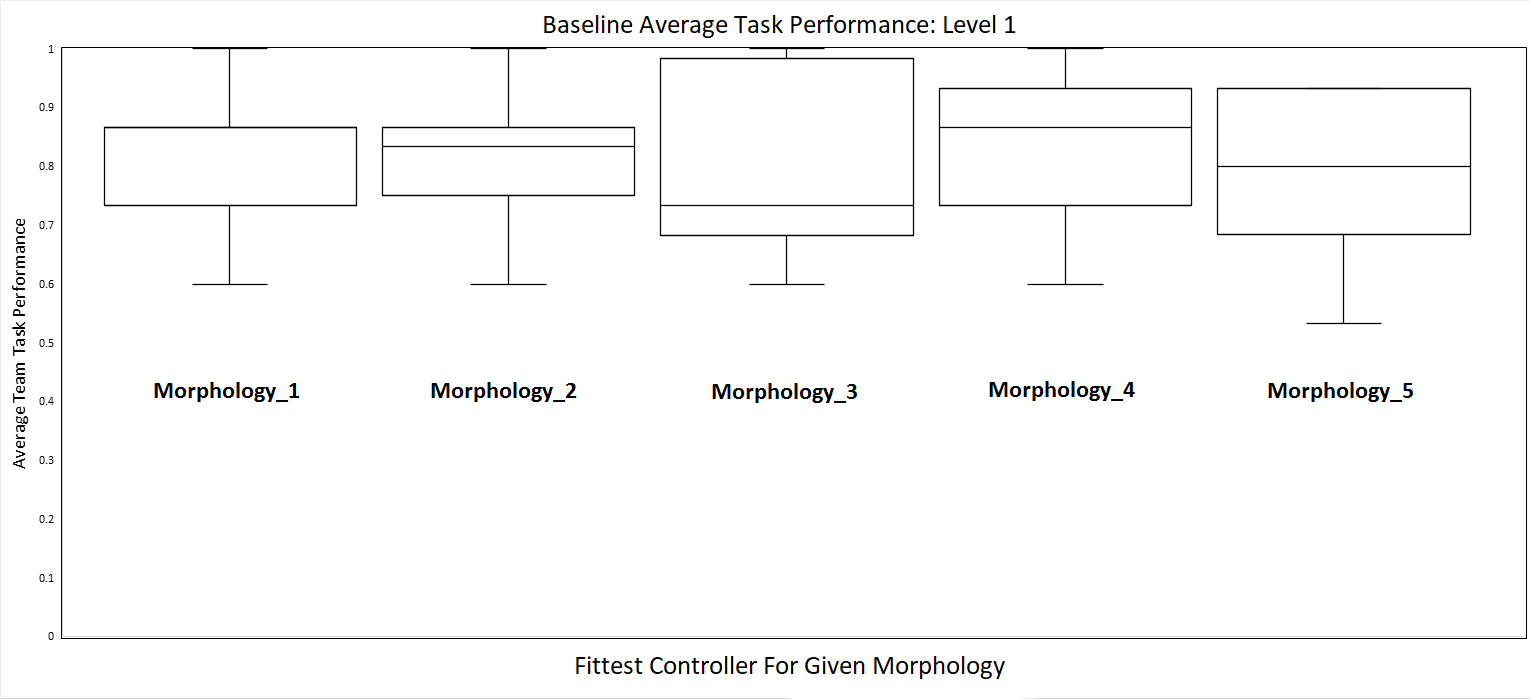
\includegraphics[width=\textwidth]{Baseline_Level_1.png}
	\end{minipage}
	\begin{minipage}{0.5\textwidth}
		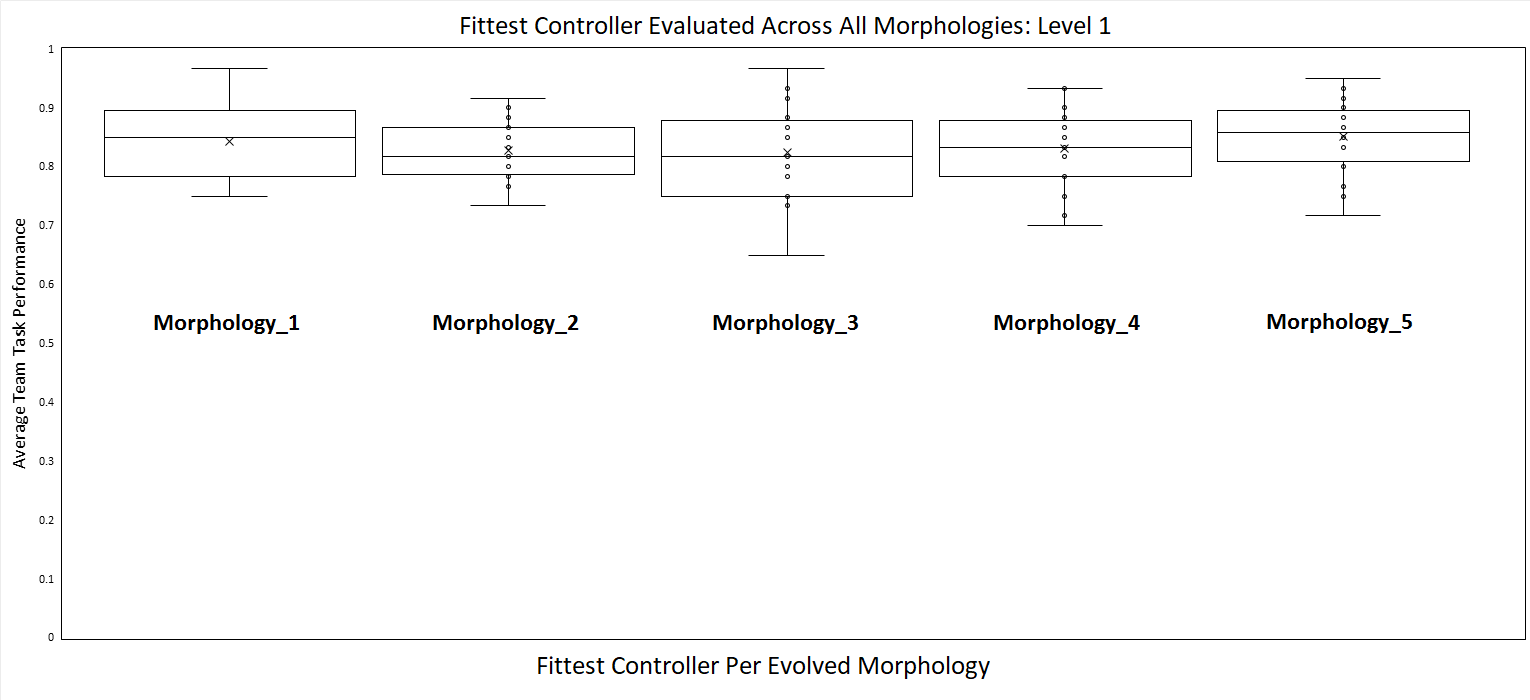
\includegraphics[width=\textwidth]{Average_Eval_Level_1.png}
	\end{minipage}
\caption{\textit{Left column:} Baseline task performance for evolved controllers (\textit{task level 1})
given morphologies $1-5$ (depicted from left to right).
\textit{Right column:} Average task performance given the fittest controller evolved
for each respective morphology ($1-5$, shown left to right) evaluated across all other morphologies.
For example: Left-most plot is average task performance of fittest controller evolved for
morphology $1$, evaluated across morphologies $2-5$.  Right-most plot is the average task performance
of fittest controller evolved for morphology $5$, evaluated across morphologies $1-4$.}\label{fig:level1results}
\end{figure*}

\begin{figure*}[t]
	\begin{minipage}{0.5\textwidth}
		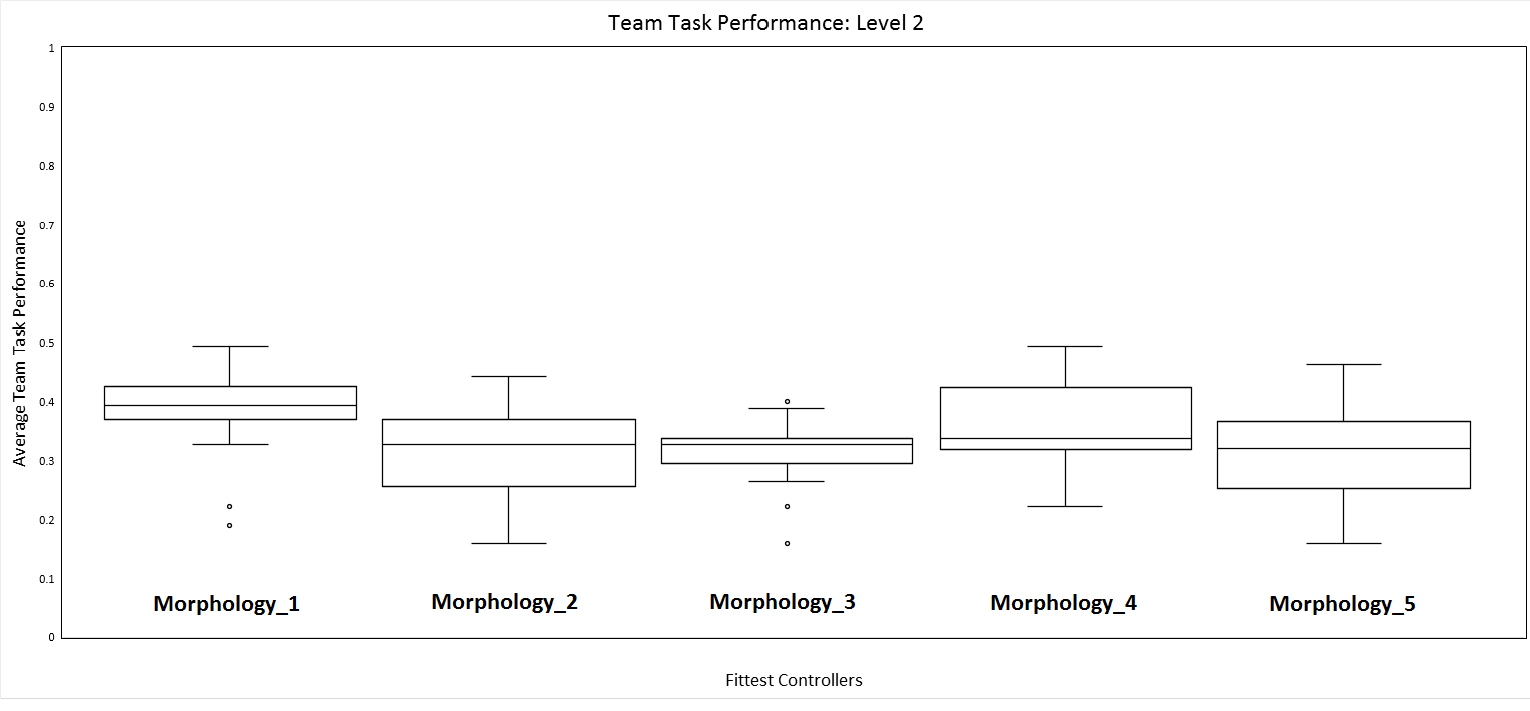
\includegraphics[width=\textwidth]{Baseline_Level_2.png}
	\end{minipage}
	\begin{minipage}{0.5\textwidth}
		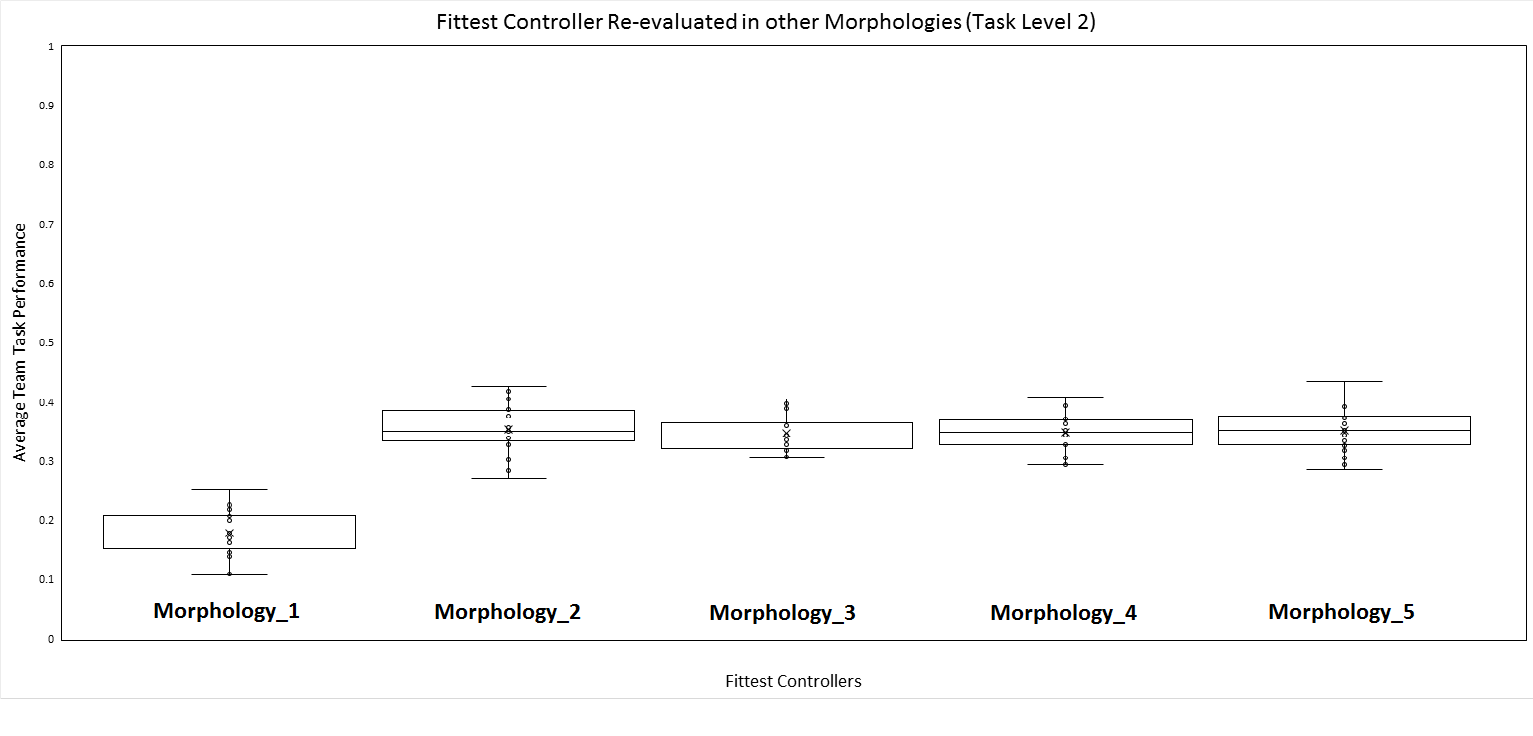
\includegraphics[width=\textwidth]{Average_Eval_Level_2.png}
	\end{minipage}
\caption{\textit{Left column:} Baseline task performance for evolved controllers (\textit{task level 1})
given morphologies $1-5$ (depicted from left to right).
\textit{Right column:} Average task performance given the fittest controller evolved
for each respective morphology ($1-5$, shown left to right) evaluated across all other morphologies.
For example: Left-most plot is average task performance of fittest controller evolved for
morphology $1$, evaluated across morphologies $2-5$.  Right-most plot is the average task performance
of fittest controller evolved for morphology $5$, evaluated across morphologies $1-4$.}\label{fig:level2results}
\end{figure*}

\begin{figure*}[t]
	\begin{minipage}{0.5\textwidth}
		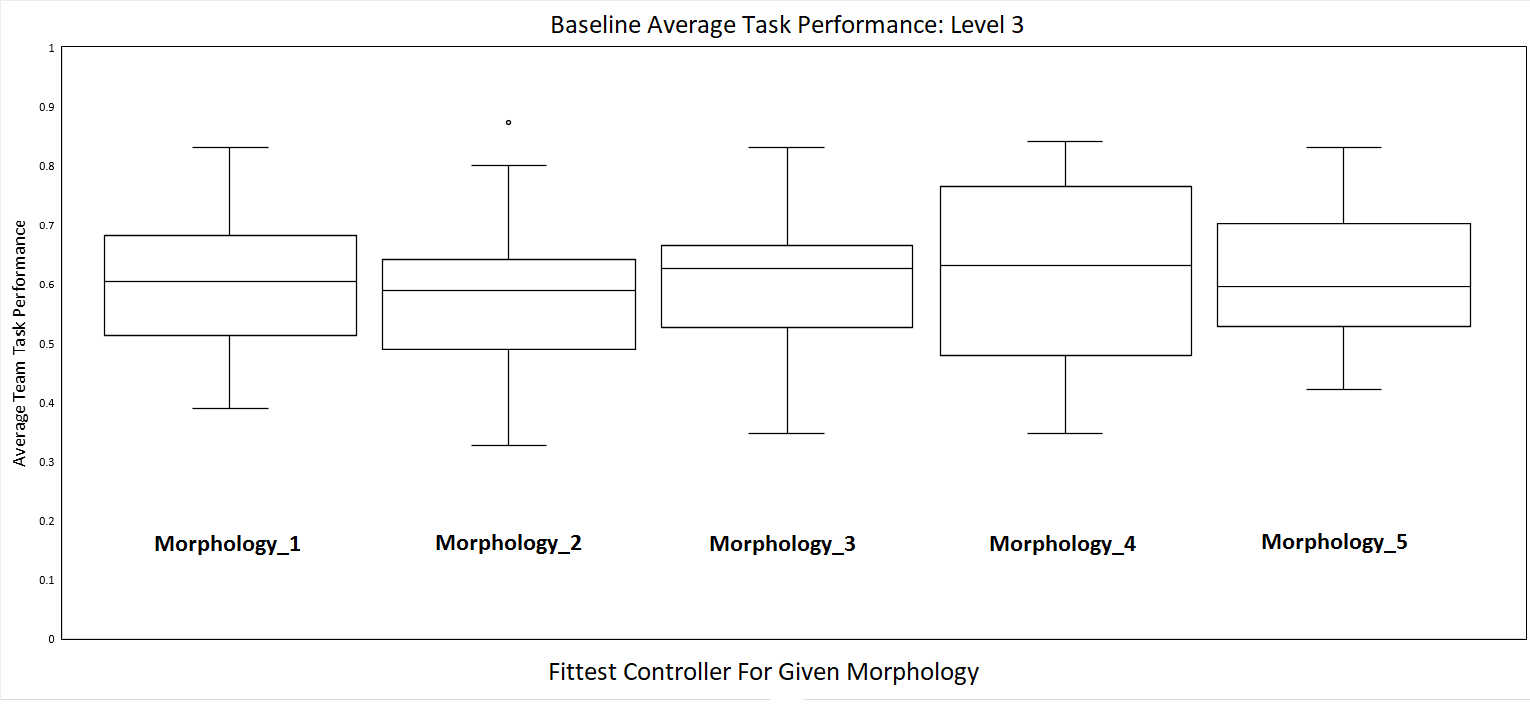
\includegraphics[width=\textwidth]{Baseline_Level_3.png}
	\end{minipage}
	\begin{minipage}{0.5\textwidth}
		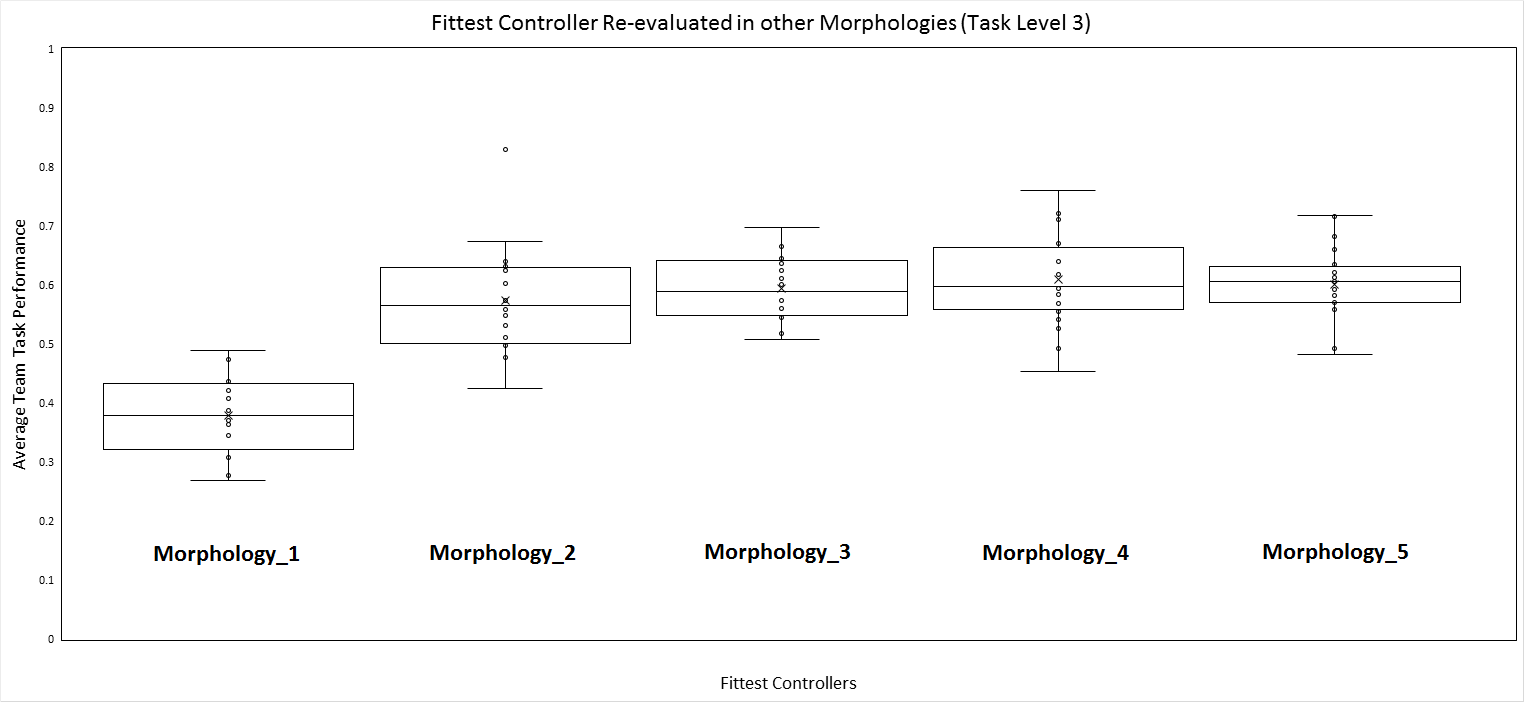
\includegraphics[width=\textwidth]{Average_Eval_Level_3.png}
	\end{minipage}
\caption{\textit{Left column:} Baseline task performance for evolved controllers (\textit{task level 1})
given morphologies $1-5$ (depicted from left to right).
\textit{Right column:} Average task performance given the fittest controller evolved
for each respective morphology ($1-5$, shown left to right) evaluated across all other morphologies.
For example: Left-most plot is average task performance of fittest controller evolved for
morphology $1$, evaluated across morphologies $2-5$.  Right-most plot is the average task performance
of fittest controller evolved for morphology $5$, evaluated across morphologies $1-4$.}\label{fig:level3results}
\end{figure*}


For each evolution phase of an experiment set, the average maximum task performance
of controllers evolved for a given morphology and level of task complexity, was recorded.

Specifically, this task performance was calculated by running the absolute fittest controller
evolved after $20$ evolutionary runs (for a given a morphology and task level),
in the same morphology over $20$ non-evolutionary runs (baseline calculations in \ref{sec:experiment_outline}).

This is previously referred to as the baseline average score for a specific controller (section \ref{sec:experiment_outline}).

This is presented in figures \ref{fig:level1results}, \ref{fig:level2results} and \ref{fig:level3results}
(left column), where controllers were evolved given morphologies $1$-$5$ (table \ref{tab:morphConfigs}).
In figures \ref{fig:level1results}, \ref{fig:level2results} and \ref{fig:level3results} (left column),
these results are presented from left to right.

For example, average task performance results for morphology $1$ are plotted on the left-most side
and average task performance results for morphology $5$ are plotted on the right-most side.

For each evaluation phase of an experiment set, the fittest controller evolved for a given morphology and task complexity
level was evaluated across all other morphologies (for the same level of task complexity), and an
average task performance computed over $20$ runs.

These morphological evaluation results are presented in figures \ref{fig:level1results}, \ref{fig:level2results}
and \ref{fig:level3results} (right column).

Each of the five plots (from left to right) in each figure corresponds to the fittest controller evolved for each of the
five morphologies and re-evaluated in all other morphologies.  
For example, the left-most plot presents
the average task performance of the fittest controller evolved in morphology $1$ and re-evaluated on morphologies $2-5$.

Where as, the right-most plot presents the average task performance of the fittest controller evolved given morphology $5$
(as the initial sensory configuration) and re-evaluated on morphologies $1-4$.

To gauge the impact of a given team morphology (table \ref{tab:morphConfigs})
in company with a given level of task complexity (table \ref{tab:taskComplexity}),
the \textit{t-test} \cite{FlanneryTeukolsky1986} ($p < 0.05$),
was applied in pair-wise comparisons between sets of controller evolution
results\footnote{Statistical test results for pair-wise comparisons for the fittest evolved controllers
(for a given morphology) tested in each other morphology (individually) is online at:
\url{https://github.com/not-my-name/SSCI_Paper_Appendix}}
(figures \ref{fig:level1results}, \ref{fig:level2results} and \ref{fig:level3results}, left column).

Within each given level of task complexity, no statistically significant difference was found between
controllers evolved given morphologies $1-5$ (controller evolution experiments $1-5$).

Controller evolution experiments $1-4$ were those implementing controller evolution in fixed sensory
configurations (morphologies $1-4$).  Where as, controller evolution experiment $5$ used morphology $5$
as the initial sensory configuration and subsequently co-adapted behavior (controller) and morphology
(complement of sensors).

The lack of statistical difference between controllers evolved given morphologies $1-4$ (table \ref{tab:morphConfigs})
indicates that these sensory configurations were not sufficiently different so as to result in
significantly different average maximum task performances.

Also, the lack of any significant difference between the average maximum task performance of controllers
evolved given morphologies $1-4$ and behavior-morphology co-adaptation (starting with morphology $5$),
supports previous results demonstrating that behavior-morphology co-adaptation
yields at least comparable task performance benefits (compared to fixed morphology controller evolution)
in collective behavior tasks \cite{HewlandNitschke2015}.

However, to address this study's main objective it was necessary to ascertain the morphological robustness
of the fittest controller evolved in each morphology when re-evaluated in all other morphologies.

To gauge the morphological robustness of the fittest controllers evolved for a given morphology ($1-5$),
and a given task complexity, we applied the t-test in pair-wise comparisons of two result
data sets.  

First, the average maximum task performances yielded by controller evolution in morphologies
$1-5$ and second, the average maximum task performances yielded from evaluating the fittest controller
evolved for a given morphology in all other morphologies (section \ref{subsec:expDesign}).
%Thus, we also used two-way ANOVA tests to measure the impact of task complexity and re-evaluating the fittest
%controller evolved for each morphology on all morphologies (in comparison to controller evolution results).

Statistical test results indicated no significant difference (with one exception) between average task performance results
yielded by baseline calculations and morphological evaluation experiments for all task complexity levels.

Specifically, the average maximum task performance yielded by controllers evolved given morphologies $2$-$5$
(figures \ref{fig:level1results}, \ref{fig:level2results}, \ref{fig:level3results}, left column) was not
significantly lower than the average task performance yielded by the fittest controllers
(evolved in morphologies $1-5$), and then re-evaluated on other morphologies
(figures \ref{fig:level1results}, \ref{fig:level2results}, \ref{fig:level3results},
right column).  

The exception was morphology $1$ in task complexity levels $2$ and $3$.

In these tasks, the fittest controller evolved for morphology $1$, yielded a significantly higher average
baseline task performance than that yielded when this fittest controller was evaluated in
morphologies $2-5$.

%Statistical test results are summarized in tables \ref{tab:anovaL1}, \ref{tab:anovaL2}
%and \ref{tab:anovaL3} for task complexity levels $1$, $2$ and $3$, respectively,
%and include performance results comparisons between controller evolution and
%morphological re-evaluation experiments with respect to task complexity and morphology.

Hence, these results indicate that controllers evolved by HyperNEAT for a given morphology
(table \ref{tab:morphConfigs}), overall have the capacity to continue to effectively operate
when transferred to other morphologies.

This result was found to hold for all four of the five morphologies that controllers were evolved for,
and for all levels of task complexity tested (table \ref{tab:taskComplexity}).
%thus demonstrating the morphological robustness of HyperNEAT evolved controllers.

The efficacy of HyperNEAT for evolving morphologically robust controllers is further supported
by the controller evolution experiments that used morphology $5$ (section \ref{sec:experiments}).

In this case, the number of sensors was adapted meaning that team behavior and
morphology were co-adapted.

Specifically, these controller evolution experiments began with the sensory configuration of
morphology $5$ (table \ref{tab:morphConfigs}) and enabled and disabled sensor connections to
better couple morphology with the evolved controller.  

Hence, the fittest controller evolved in this case often corresponded to a sensory configuration
dissimilar to morphology $5$ (the initial sensory configuration).

Results indicated that the fittest controller evolved for morphology $5$, when evaluated across
other morphologies, yielded an average task performance that was statistically comparable to
the average baseline task performance yielded given morphology $5$.

This result was observed for all three task complexity levels
(figures \ref{fig:level1results}, \ref{fig:level2results}, and \ref{fig:level3results}, right column).

Thus, controllers evolved for fixed morphologies ($1-4$, table \ref{tab:morphConfigs}), were
found to be \textit{morphologically robust}, as there was no significant difference in average maximum
task performance when the fittest controller (evolved for morphology $1-4$), was evaluated using other
morphologies.

Furthermore, the fittest controller evolved for an adaptive morphology ($5$, table \ref{tab:morphConfigs}),
was similarly found to be morphologically robust, given that the average maximum task performance
yielded when this fittest controller was evaluated in other morphologies ($1-4$), was comparable to
the average maximum task performance yielded from morphology $5$ controller evolution experiment (baseline average fitness).

This is theorized to be a result of the complexity of co-adapting effective controller-morphology
couplings \cite{PfeiferBongard2006} within limited periods of artificial evolution ($100$ generations in these experiments,
table \ref{tab:simParameters}), offset by the transference of evolved
\textit{connectivity patterns} \cite{GauciStanley2010} as functional controllers across varying
robot morphologies  \cite{RisiStanley2013}.

Such connectivity patterns encode behaviors that do not rely upon specific sensory-motor mappings in
controllers and thus do not necessitate specific task environment configurations,
such as specific numbers of agents or objects.

This in turn facilitates the transfer of controllers across varying team morphologies
\cite{verbancsics_evolving_2010}, \cite{DidiNitschke2016SSCI}, \cite{DidiNitschke2016}.
%a benefit of HyperNEAT elucidated from such collective behavior transfer research was found to be its capability
%to evolve connectivity patterns between the sensory-motor layers of agent controllers
%that are broadly applicable to collective behavior tasks of varying complexity.
%versus adaptive morphologies had no significant impact on the
%morphological robustness of HyperNEAT evolved controllers (gauged in terms of average team task performance)
%for all morphologies tested.  %This result was observed for all levels of task complexity tested.

These results are corroborated by related work \cite{RisiStanley2013}, \cite{WatsonNitschke2015SSCI},
and contribute further empirical evidence that HyperNEAT yields significant benefits in
evolving robot controllers that effectively operate in other morphologies.

That is, this study further demonstrated HyperNEAT's capability to exploit geometric properties
such as regularity, repetition and symmetry in robot morphology and environment \cite{StanleyDAmbrosioGauci2009},
where such modularity and geometric properties are encoded in evolved connectivity patterns.

This is prevalent in this study, as the configuration of sensors on each robot's periphery was
symmetrical for all morphologies tested (section \ref{sec:embodiment}).
\hl{Not sure if the above is correct since Morph 5 was a random distribution}


Also, the collective construction task required that blocks be connected together in a repeated manner in a symmetrical bounded
simulation environment ($20$x$20$ units, table \ref{tab:simParameters}).

The capability of HyperNEAT evolved controllers to operate in different morphologies is further
supported by other research \cite{verbancsics_evolving_2010}
demonstrating that evolved indirect sensory-motor mappings can
encapsulate effective behaviors with relatively few task environment and robot
geometric relationships, such as desired positions and angles between robots and different object types.

The efficacy of HyperNEAT for evolving morphologically robust controllers for collective behavior
tasks of varying complexity is also supported by related research in \textit{multi-agent policy transfer}
\cite{verbancsics_evolving_2010}, \cite{DidiNitschke2016SSCI}, \cite{DidiNitschke2016}.

Policy transfer methods facilitate the transfer of behaviors across tasks of increasing
complexity or between dissimilar tasks.  

Such studies have demonstrated that HyperNEAT is an effective
method for evolving behaviors in one collective behavior task and then transferring the evolved behavior
to a related but more complex task (for example, where robots have more complex sensory-motor configurations
to process increased task complexity) with relatively little loss in average team task performance.
%That is, HyperNEAT evolves CPPNs representing controllers of varying complexity with their own symmetries
%and regularities which are able to effectively exploit varyingly complex robot (agent) sensory-motor configurations.
%This in turn, often significantly boosts the efficacy of evolved collective behaviors \cite{DAmbrosio2013}.

However, we hypothesize that the morphological robustness of HyperNEAT evolved controllers demonstrated across all
morphologies tested (table \ref{tab:morphConfigs}) and all levels of task complexity
(table \ref{tab:taskComplexity}) was facilitated by the use of morphologically and behaviorally homogenous teams.

Specifically, one controller was evolved for all robots in a team and all robots used the same sensory configuration, meaning
all robots had the same \textit{collective behavior geometry} \cite{DAmbrosioLehmanStanley2010}.
This in turn simplified the transfer of evolved controllers across varying morphologies with no significant degradation
in average task performance.

Hence, overall, this study's results demonstrate that HyperNEAT is an appropriate method for evolving
morphologically robust controllers.  

That is, controllers that are fully functional in a range of team morphologies.

In order to ascertain how well HyperNEAT evolved controllers generalize, ongoing research is evaluating
the evolution of morphologically robust behaviors in behaviorally and morphological heterogenous teams
for complex collective behavior tasks that are irregular and without repetition or symmetry.

Furthermore, current research is comparing HyperNEAT to related evolutionary approaches that have demonstrated
controllers able to accomplish multiple disparate tasks in dynamic environments
\cite{IzquierdoTorres2008}, as well as direct encoding neuro-evolution methods such as NEAT \cite{StanleyMiikkulainen2002}.

